% !TEX root = ../../thesis.tex

\section{Design Principles} \label{designPrinciples}

In order to address the problems mentioned in the \nameref{problemStatement} (\ref{problemStatement}) section, we adopted and implemented the following design principles.

\subsection{No foreign code execution}

There is no foolproof way of entirely securing a piece of software; even the most mature platforms and operating systems sometimes end up vulnerable to security exploits. However, without the ability to execute code on a platform, it is not directly possible to take advantage of vulnerabilities, even when there is one. Furthermore, the nature of Intertext allowed us to adopt disallowing code execution as a design principle. Intertext clients only accept UIUDL code, which is in XML and is not executable. Should a server send anything else, Intertext clients will simply ignore it. Thus, we can guarantee security for the users, regardless of the platform they are using the Intertext client on.

\subsection{Transparency}

Privacy is a common concern among users; primarily due to the recent scandals and data leaks, people started getting more conscious about their data. There is an increasing demand for users to be more in control and be aware of what is exposed and what is not. In order to address this burning need, we adopted transparency as a design principle. 

The most prominent way of achieving this is to have Intertext clients be in control of all interactions with the device and with external sources and keep logs in order to make them transparent to the user. The above-mentioned principle that no foreign code will be executed goes hand-in-hand in achieving this, as it would be unrealistic to expect complete control as it would be a non-deterministic approach. A good analogy would be to think of Intertext clients as an API endpoint that runs on users devices and exposes fundamental interactions with the host device and external networks through an API in a fully controlled manner. An application could "instruct" the Intertext client via IUIDL to perform some actions, such as making a network request, storing data, and accessing the local storage. Intertext client will then block this action until the user grant permission and keep logs every time before performing an action (Fig \ref{fig:permission_flow})

\begin{figure}
  \centering
  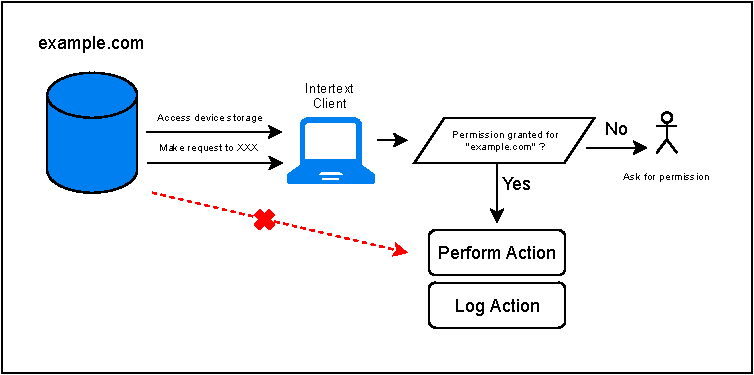
\includegraphics[width=13cm]{thesis/paper/images/permission.pdf}
  \caption{A diagram showing the permission flow}%
  \label{fig:permission_flow}%
\end{figure}


\subsection{Black-box Components as Building Blocks}

Intertext adopts a component based approach, we provide a set of components for developers to use to build their applications with. Each component accepts a set of properties, which gives them certain functionality or appearance. Developers are to use these components through IUIDL. For example, the IUIDL code below (at Figure \ref{fig:iuidl_buttons}) and it's output for Intertext web version (at Figure \ref{fig:iuidl_buttons_output}) shows some of the properties that \textit{button} component accepts. Layout properties such as  \textit{marginButton} allows positioning of the buttons to be customised, \textit{intent} properties gives the button a different look based on the use-case, properties like \textit{disabled} can alter its behaviour and so on.

\begin{figure}
\begin{minipage}{\linewidth}
\begin{lstlisting}[language=html]
<h3>Buttons</h3>

<grid cols="[1,1]">
  <block>
    <button marginBottom="2">default</button>
    <button marginBottom="2" disabled="true">disabled</button>
  </block>
  <block>
    <button marginBottom="2" intent="default">default</button>
    <button marginBottom="2" intent="primary">primary</button>
    <button marginBottom="2" intent="error">error</button>
    <button marginBottom="2" intent="warning">warning</button>
    <button marginBottom="2" intent="success">success</button>
    <button marginBottom="2" intent="info">info</button>
  </block>
</grid>
\end{lstlisting}
\end{minipage}
\caption{UIUDL that renders buttons in several states}%
\label{fig:iuidl_buttons}%
\end{figure}

\begin{figure}
  \centering
  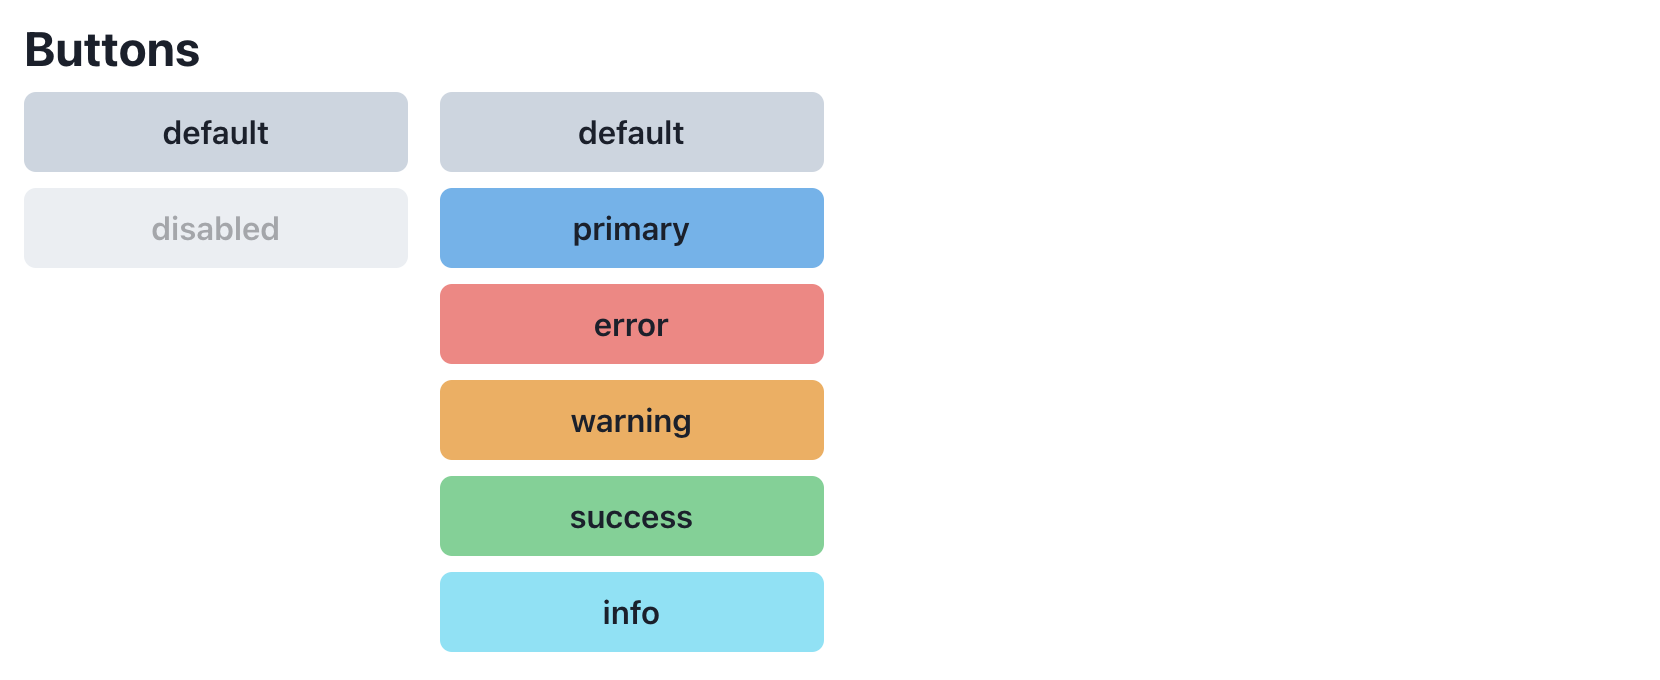
\includegraphics{thesis/paper/images/buttons.png}
  \caption{Output of IUIDL at Figure \ref{fig:iuidl_buttons} on Intertext web client}%
  \label{fig:iuidl_buttons_output}%
\end{figure}

However other than properties that components accepts, they cannot be modified or altered by the developer. The main motive behind this principle is standardisation. When all Intertext applications uses the same set of components, we can control how they look and how they are implemented, and ensure certain behavioural and visual aspects to bring the benefits in order to solve some of the problems mentioned in the \nameref{problemStatement} section.

Consistency is one of the most important benefit that this principle enables. A standard look and feel for components helps users to never get disoriented across applications, and recognise similar patterns easily. Another benefit is customisability, it is only possible to create one-size-fits-all themes that applies to every component in every application when all the applications uses components that are built in the same way. Another thing that comes to mind is accessibility. We established in section \ref{problemStatement} that accessibility is a big issue that not all developers choose to address. This principle allows us to take this responsibility from the developers hands by providing accessible components as building blocks. 

\begin{figure}[H]
  \centering
  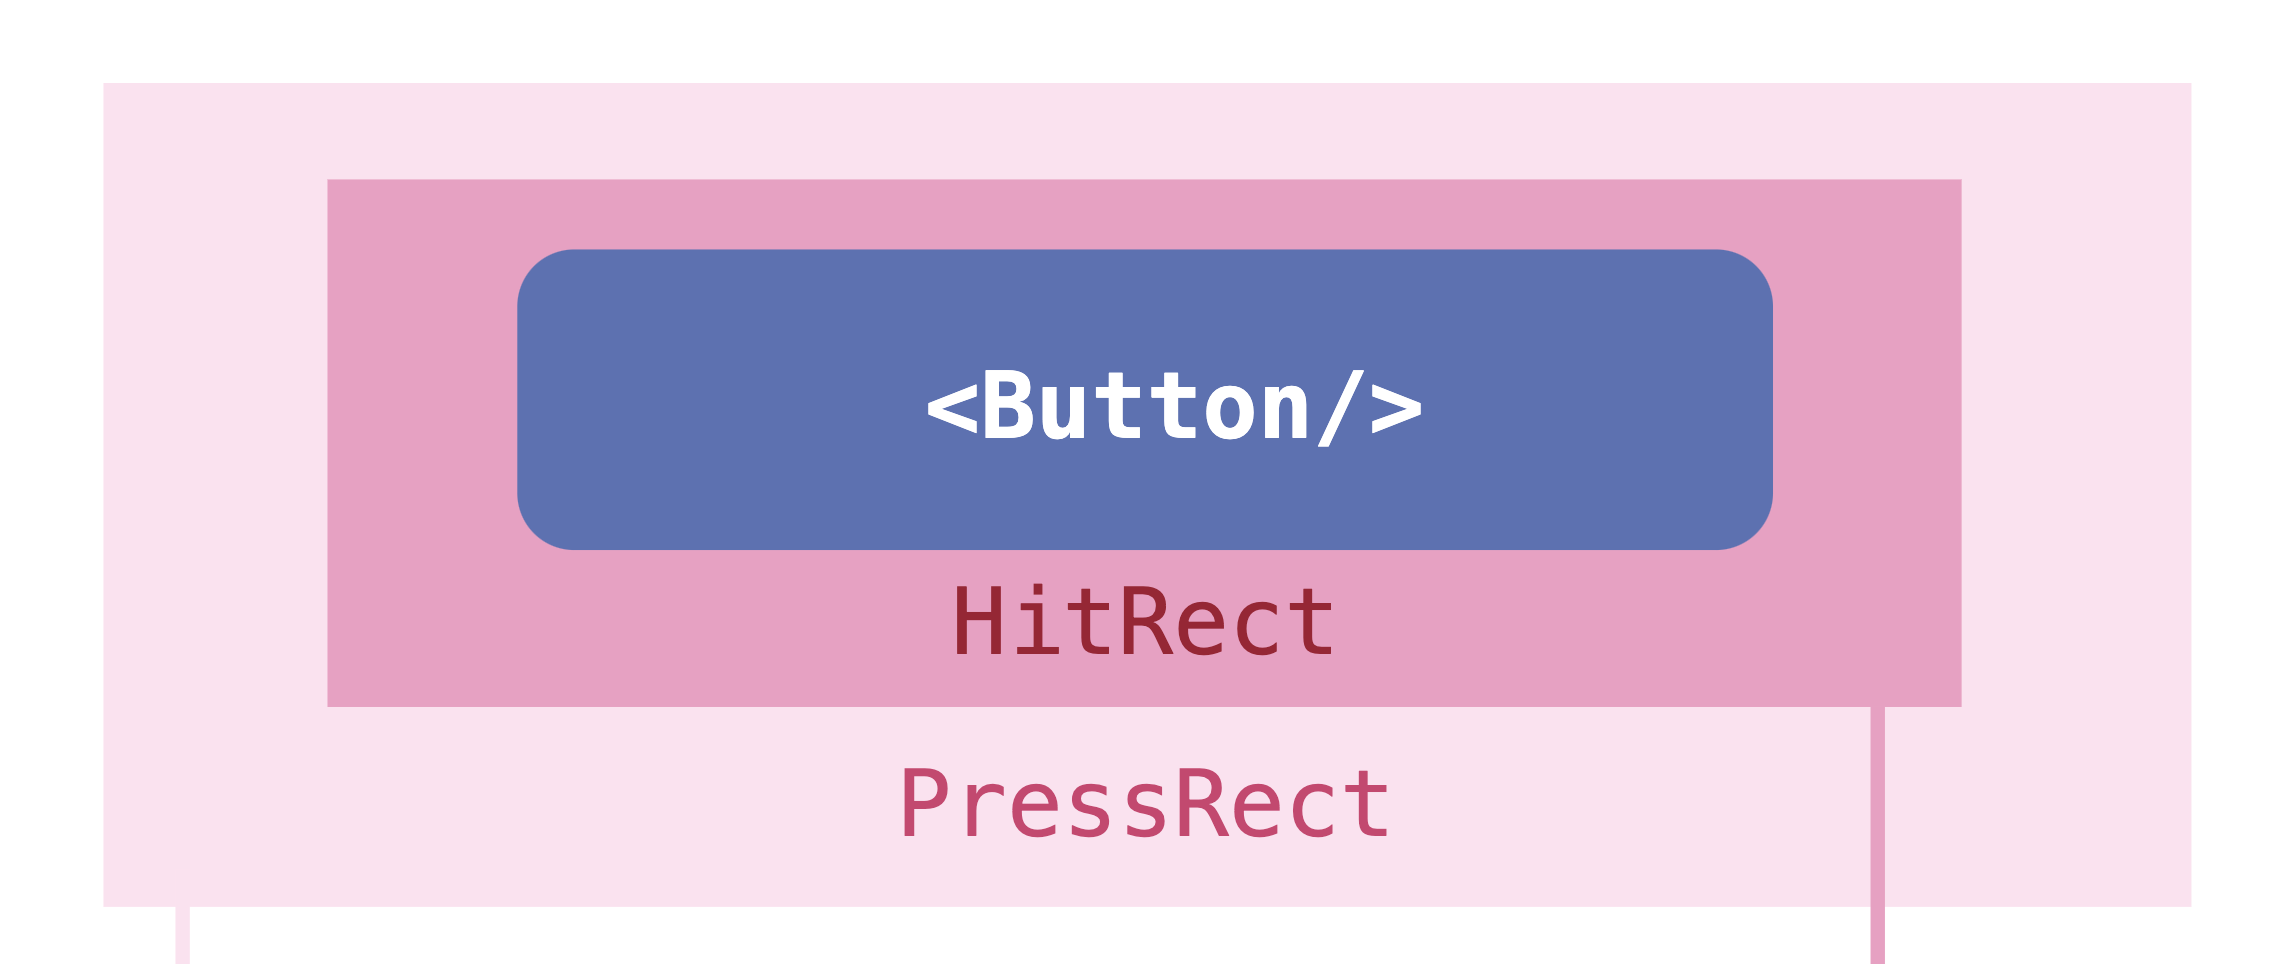
\includegraphics[width=13cm]{thesis/paper/images/pressable.png}
  \caption{Diagram that shows the implementation of Pressable component in React Native (reactnative.dev/docs/pressable)}%
  \label{fig:pressable}%
\end{figure}

Last but not least, this principle was crucial to achieve cross-device compatibility. The appearance and behaviour of components differs between implementations of the Intertext clients. For instance, the \textit{button} component on the web version needs not to be too big as clicks are precise, it requires a hover and focus state and so on. For a touch interface however, it needs to be bigger, and handle the caveat of having less precision by accepting hits on an area around it as seen in figure \ref{fig:pressable}. Every feature that components have needs to be supported as much as possible on different platforms that has different requirements. Having components with a fixed set of features allowed us to implement them all for different Intertext clients.

\subsection{Shared syntax between clients}

We designed IUIDL to be a generic markup language, agnostic of any platform or interaction type, and be based purely on XML so it could be consumed by all clients. This approach has many advantages, both for developers and users. It allows developers to create universal applications; once they start serving an Intertext application through an endpoint, any Intertext endpoint can consume the application through that endpoint. Moreover, it helps create a continual experience for the user; given that there is a shared layout system, UI elements will look and feel the same between Intertext clients. Figure \hl{TODO} and \hl{TODO} shows the similarities between Intertext web client and the command-line client.

\hl{TODO Add screenshots that shows similarities between the web version and the cli version}

Also, this approach allows existing Intertext applications to adopt to new Intertext clients as they are built in the future. At the time of this paper, Intertext web client and command-line client is ready, but as mentioned in the \hl{TODO: Future Work} section, more Intertext clients are on the way. Thanks to this principle, Intertext clients will have immediate availability for the upcoming Intertext clients.
